\documentclass[usepdftitle=false, compress]{beamer}

\usepackage{calc}
\newlength{\leftstart}
\newlength{\topstart}
\setlength{\leftstart}{\hoffset + \oddsidemargin + 1in}
\setlength{\topstart}{\voffset + \topmargin + 1in}

\newlength{\figfour}

\usepackage{etex}
\usepackage{etoolbox}
\usepackage[absolute,overlay]{textpos}
\usepackage{fancybox}

\usepackage{xcolor}
\definecolor{myblue}{rgb}{0,0.4,0.7}
\definecolor{myred}{rgb}{0.7,.1,.1}
\definecolor{mygray}{rgb}{0.7,0.7,0.7}
\definecolor{mygreen}{rgb}{0,0.8,0.1}

\useinnertheme{circles}

\DeclareMathOperator*{\argmin}{arg\,min}

\mode<presentation>{
  \setbeamertemplate{navigation symbols}{}
	\usepackage{lmodern}
	\setbeamercolor{title}{fg=myblue}
	\setbeamercolor{frametitle}{fg=black}
}

\newcommand{\myemph}[1]{{\color{myblue}#1}}

% Drawing with TiKz
\usepackage{tikz}
\usetikzlibrary[positioning]
\usetikzlibrary{patterns}
\usetikzlibrary{backgrounds}
\usetikzlibrary{calc}
\usetikzlibrary{shapes.geometric}
\usetikzlibrary{shapes.arrows}
\usetikzlibrary{arrows}
\usetikzlibrary{calc,positioning,shapes,chains,mindmap,trees,decorations}

\usepackage{rotating}
\usepackage[utf8]{inputenc}
\usepackage[english]{babel}
\usepackage{amssymb,amsmath,amsthm}
\usepackage{graphicx,graphics}
\usepackage{multicol}
\usepackage{multirow}
\usepackage{tabularx}
\newcolumntype{Y}{>{\centering\arraybackslash}X}
\newcolumntype{Z}{>{\raggedright\arraybackslash}X}
\newcolumntype{W}{>{\raggedleft\arraybackslash}X}

\usepackage{array}
\newcolumntype{L}[1]{>{\raggedright\let\newline\\\arraybackslash\hspace{0pt}}m{#1}}
\newcolumntype{C}[1]{>{\centering\let\newline\\\arraybackslash\hspace{0pt}}m{#1}}
\newcolumntype{R}[1]{>{\raggedleft\let\newline\\\arraybackslash\hspace{0pt}}m{#1}}

\usepackage{pgfgantt}

\usepackage[pdf]{pstricks}

\usepackage[absolute,overlay]{textpos}

\usepackage{pifont}% http://ctan.org/pkg/pifont
\newcommand{\cmark}{\color{mygreen}\ding{51}}%
\newcommand{\xmark}{\color{myred}\ding{55}}%
\newcommand{\mehhh}{\color{mygray}$\sim$}%

\newcommand{\prog}{ $\vartriangleright$ }

\usepackage{enumitem}
\setitemize{label=\usebeamerfont*{itemize item}%
  \usebeamercolor[fg]{itemize item}
  \usebeamertemplate{itemize item}}

\newenvironment{compitem}{\begin{itemize}[noitemsep,topsep=0pt,parsep=0pt,partopsep=0pt]}{\end{itemize}}

\newcommand{\wholeslide}[1]{{
\usebackgroundtemplate{\includegraphics[width=\paperwidth]{#1}}
\begin{frame}[plain]
\end{frame}
}}
\usepackage{soul}

\makeatletter
\def\imod#1{\allowbreak\mkern7mu{\operator@font mod}\,\,#1}
\def\m#1{\allowbreak\mkern10mu({\operator@font mod}\,\,#1)}
\makeatother

\newcommand{\summary}[5]{%
	\begin{frame}
		\begin{itemize}
			\item {\color{#1}Single-cell biology}
			\item {\color{#2}Trajectory inference}
			\item {\color{#3}Network inference}
			\item {\color{#4}Benchmarking}
			\item {\color{#5}Practical implications}
		\end{itemize}
	\end{frame}
}
\newcommand{\topright}[1]{%
\begin{textblock*}{.15\linewidth}(.98\linewidth,.05\linewidth)
	\includegraphics[width=\linewidth]{figures/overview_#1.pdf}
\end{textblock*}}

\title{Modelling single-cell dynamics\\with trajectories and gene regulatory networks}

\author{Robrecht Cannoodt}

\date{}

\begin{document}

\begin{frame}[plain]
  \titlepage
  \hfill
  
\includegraphics[height=.42cm]{../fig/logos/icon_UGent_WE_EN_RGB_color}\hfill
  
\includegraphics[height=.60cm]{../fig/logos/vib_rf_inflammation_research_rgb_pos} \hfill
  \includegraphics[height=.48cm]{../fig/logos/dambi_logo} \hfill
  \includegraphics[height=.42cm]{../fig/logos/cmgg_myshort} \hfill
  
\includegraphics[height=.42cm]{../fig/logos/FWO_Logo_KleurCMYK} 
  \hfill
\end{frame}

%%%%%%%%%%%%%% SINGLE CELL BIOLOGY %%%%%%%%%%%%%%
\begin{frame}
	\frametitle{Single-cell biology \uncover<2->{is to study an organism}\\\uncover<3->{by studying the behaviour of its cells}}
	\begin{center}
		\only<2>{\includegraphics[width=\linewidth]{figures/1a_singlecellbiology}}%
		\only<3>{\includegraphics[width=\linewidth]{figures/1b_singlecellbiology}}%
		\only<4>{\includegraphics[width=\linewidth]{figures/1c_singlecellbiology}}%
	\end{center}
\end{frame}


\begin{frame}
	\frametitle{Technological advances allow high-throughput\\single-cell biology}
	\begin{center}
		\includegraphics[width=\linewidth]{figures/2_part_scaling.pdf}\\
		\flushright 		{\vspace*{-1em}\footnotesize Regev et al. 2018}
	\end{center}
  \vspace*{-2.2em}
\end{frame}

\begin{frame}
	\frametitle{Research questions}
	\begin{center}
		\only<2>{
\includegraphics[width=\linewidth]{figures/11a_fundamental.pdf}}%
		\only<3>{\includegraphics[width=\linewidth]{figures/11b_fundamental.pdf}}%
		\only<4>{\includegraphics[width=\linewidth]{figures/11c_fundamental.pdf}}%
		\only<5>{\includegraphics[width=\linewidth]{figures/11d_fundamental.pdf}}%
	\end{center}
\end{frame}

\begin{frame}
  \only<1>{\includegraphics[width=\linewidth]{figures/overview_categories.pdf}}
  \only<2>{\includegraphics[width=\linewidth]{figures/overview_categories_dots.pdf}}
  \only<3>{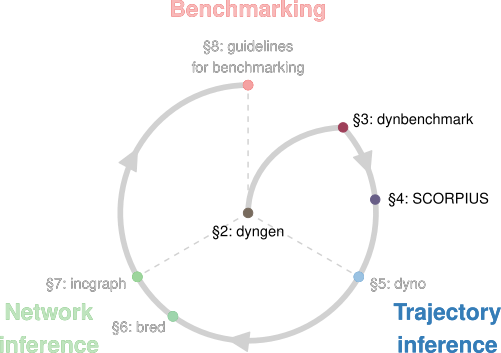
\includegraphics[width=\linewidth]{figures/overview.pdf}}
\end{frame}

%%%%%%%%%%%%%% TRAJECTORY INFERENCE %%%%%%%%%%%%%%

\begin{frame}
	\vfill
	\begin{center}
		\LARGE Trajectory inference
	\end{center}
	\vfill
\end{frame}

\begin{frame}
	\frametitle{Cells are highly dynamic entities}
	\begin{center}
		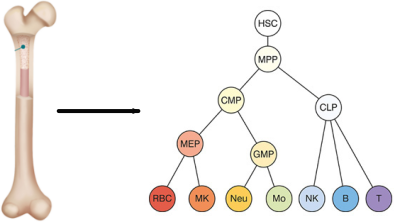
\includegraphics[width=.6\linewidth]{figures/3_dynamiccells.pdf}
	\end{center}
\end{frame}

\begin{frame}
	\frametitle{A typical trajectory inference analysis}
	\begin{center}
		\only<1>{\includegraphics[width=\linewidth]{figures/4a_trajectoryinference.pdf}}%
		\only<2>{\includegraphics[width=\linewidth]{figures/4b_trajectoryinference.pdf}}%
		\only<3>{\includegraphics[width=\linewidth]{figures/4c_trajectoryinference.pdf}}%
		\only<4>{\includegraphics[width=\linewidth]{figures/4d_trajectoryinference.pdf}}%
		\only<5>{\includegraphics[width=\linewidth]{figures/4e_trajectoryinference.pdf}}%
		\only<6>{\includegraphics[width=\linewidth]{figures/4f_trajectoryinference.pdf}}%
	\end{center}
\end{frame}

\begin{frame}
	\frametitle{dyngen: Benchmarking with \textit{in silico} cells}
	\begin{center}
		\includegraphics[width=.6\linewidth]{figures/end_part_dyngen.pdf}
	\end{center}
	\topright{ch2}
\end{frame}


\begin{frame}
	\frametitle{Benchmark of 45 trajectory inference methods}
%	\begin{center}
		\only<1>{\includegraphics[width=.9\linewidth]{figures/5a_benchmark.pdf}}%
		\only<2>{\includegraphics[width=.9\linewidth]{figures/5b_benchmark.pdf}}%
%	\end{center}
	\topright{ch3}
\end{frame}


\begin{frame}
	\frametitle{Interactive guidelines}
	\begin{center}
		\includegraphics[width=\linewidth]{figures/6_guidelines.pdf}
	\end{center}
	\topright{ch3}
\end{frame}


\begin{frame}
	\frametitle{Perspective: self-assessment in trajectory inference}
	\begin{center}
		\includegraphics[width=.8\linewidth]{figures/end_part_selfassessment.pdf}
	\end{center}
  \topright{ch8}
\end{frame}

\begin{frame}
	\frametitle{SCORPIUS: Linear trajectory inference}
	\begin{center}
		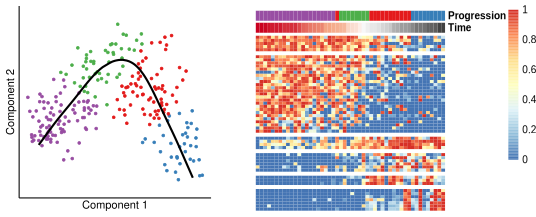
\includegraphics[width=.8\linewidth]{figures/end_part_scorpius.pdf}
	\end{center}
	\topright{ch5}
\end{frame}

\begin{frame}
	\frametitle{dyno: A toolkit for inferring and\\interpreting trajectories}
	\begin{center}
		\includegraphics[width=.9\linewidth]{figures/end_part_dyno.pdf}
	\end{center}
	\topright{ch4}
\end{frame}


%%%%%%%%%%%%%% NETWORK INFERENCE %%%%%%%%%%%%%%

\begin{frame}
	\vfill
	\begin{center}
		\LARGE Network inference
	\end{center}
	\vfill
\end{frame}

\begin{frame}
	\frametitle{Cellular dynamics is (i.a.) driven by gene regulation}
	\begin{center}
		\only<1>{\includegraphics[width=.8\linewidth]{figures/7a_generegulation.pdf}}%
		\only<2>{\includegraphics[width=.8\linewidth]{figures/7b_generegulation.pdf}}%
		\only<3>{\includegraphics[width=.8\linewidth]{figures/7c_generegulation.pdf}}%
		\only<4>{\includegraphics[width=.8\linewidth]{figures/7d_generegulation.pdf}}%
		\only<5>{\includegraphics[width=.8\linewidth]{figures/7e_generegulation.pdf}}%
		\only<6>{\includegraphics[width=.8\linewidth]{figures/7f_generegulation.pdf}}%
	\end{center}
\end{frame}

\begin{frame}
	\frametitle{Classical network inference}
	\begin{center}
		\includegraphics[width=.9\linewidth]{figures/8_networkinference.pdf}
	\end{center}
\end{frame}


\begin{frame}
	\frametitle{Case-specific network inference}
	\begin{center}
		\only<1>{\includegraphics[width=\linewidth]{figures/9a_csni_example.pdf}}%
		\only<2>{\includegraphics[width=\linewidth]{figures/9b_csni_example.pdf}}%
		\only<3>{\includegraphics[width=\linewidth]{figures/9c_csni_example.pdf}}%
		\only<4>{\includegraphics[width=\linewidth]{figures/9d_csni_example.pdf}}%
	\end{center}
	\topright{ch6}
\end{frame}

\begin{frame}
	\frametitle{bred applied to TCGA}
	\begin{center}
		\includegraphics[width=.85\linewidth]{figures/10b_tcga.pdf}
%		\only<1>{\includegraphics[width=.6\linewidth]{figures/10a_tcga.pdf}}%
%		\only<2>{\includegraphics[width=.85\linewidth]{figures/10b_tcga.pdf}}%
	\end{center}
	\topright{ch6}
\end{frame}

\begin{frame}
	\frametitle{incgraph: Optimising regulatory networks}
	\begin{center}
		\includegraphics[width=\linewidth]{figures/end_part_incgraph.pdf}
	\end{center}
	\topright{ch7}
\end{frame}

%%%%%%%%%%%%%%%%%%% BENCHMARKING
\begin{frame}
	\vfill
	\begin{center}
		\LARGE Benchmarking
	\end{center}
	\vfill
\end{frame}

\begin{frame}
	\frametitle{Essential guidelines for benchmarking\\computational tools}
	\begin{center}
		\includegraphics[width=\linewidth]{figures/end_part_guidelines.pdf}
	\end{center}
	\topright{ch9}
\end{frame}

%%%%%%%%%%%%%% IMPLICATIONS %%%%%%%%%%%%%%


\begin{frame}
	\frametitle{Practical implications}
	\begin{itemize}
		\item<2-> Fundamental research in single-cell analyses \\
		  \uncover<3->{\begin{center}\includegraphics[width=.7\linewidth]{figures/11d_fundamental.pdf}\end{center}}
		\item<4-> Benchmarking
		\item<5-> R \& tidyverse
	\end{itemize}
  \topright{all}
\end{frame}


\end{document}